\documentclass[../thesis.tex]{subfiles}

\begin{document}

\chapter{The Daya Bay experiment}
\label{chap:experim}

\section*{Introduction}

The Daya Bay experiment was designed to measure $\theta_{13}$ by observing the antineutrinos produced by the six 2.9~GW$_{\text{th}}$ nuclear reactors of the Daya Bay and Ling Ao power plants, located near Shenzhen in southern China. A total of eight functionally identical antineutrino detectors (ADs) were deployed, each containing a target of 20~tons of gadolinium-doped liquid scintillator (GdLS). Four of the ADs were evenly divided among two near halls ($\sim$350-600~m baselines from the cores), and the remaining four were placed in a single far hall ($\sim$1500-1950~m baselines). Shielding from cosmic rays was provided by $\sim$100~m and $\sim$300~m, respectively, of mountainous overburden at the near and far halls. The ADs in each hall were immersed in instrumented water pools which provided shielding from ambient radioactivity and detection of Cerenkov radiation from atmospheric muons. Redundant detection of muons, as well as directional information, were made available by resistive plate chambers (RPCs) laid on top of the water pools. This chapter provides a detailed account of the layout, detectors, and shielding/vetoing system of the experiment.

\section{Site layout}
\label{sec:expLayout}

\begin{figure}[ht]
  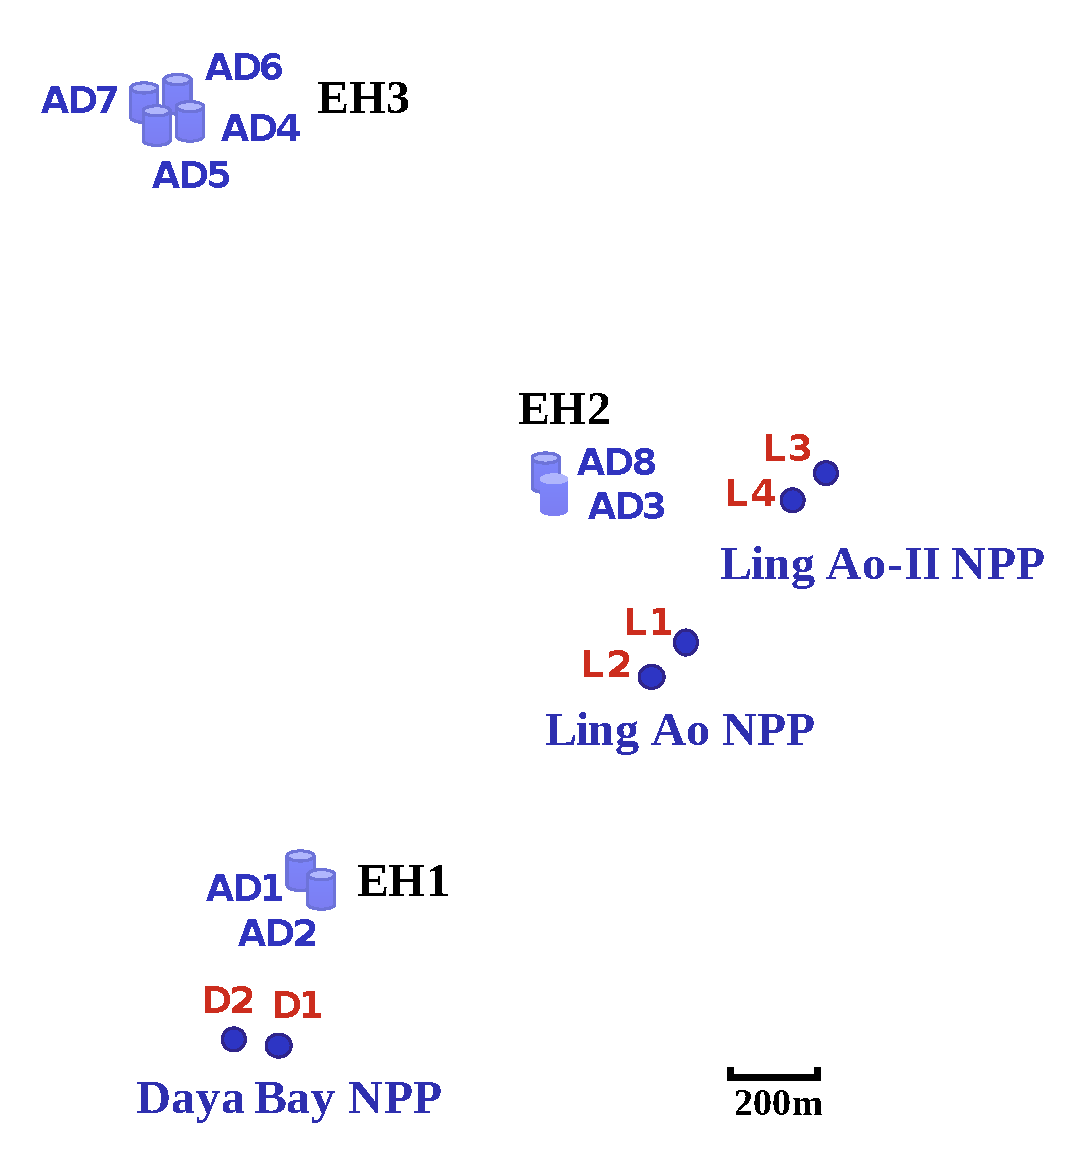
\includegraphics[scale=0.4]{inkLayout.pdf}
  \caption{The layout of the Daya Bay experiment. Modified from \cite{SideBySide}.}
  \label{fig:layout} 
\end{figure}

As shown in \autoref{fig:layout}, the power reactors are divided into three nuclear power plants (NPPs) of two cores each. One of the clusters makes up the Daya Bay NPP (cores D1 and D2), while the other two adjacent clusters make up the Ling Ao (L1 and L2) and Ling Ao-II (L3 and L4) NPPs. EH1 is located around 350~m from the Daya Bay NPP, while EH2 is roughly 500~m from the two Ling Ao NPPs. The far hall, EH3, in turn is located about 1900~m from the Daya Bay NPP and 1500~m from the Ling Ao NPPs. The exact baselines are given in \autoref{tab:expBaselines}.

\begin{table}[ht]
  \begin{tabular}{lcrrrrrr}
    \toprule
    \multicolumn{2}{c}{} & \multicolumn{6}{c}{Reactor baseline [m]} \\
    \cmidrule{3-8}
    Hall & Detector & \multicolumn{1}{c}{D1} & \multicolumn{1}{c}{D2} & \multicolumn{1}{c}{L1} & \multicolumn{1}{c}{L2} & \multicolumn{1}{c}{L3} & \multicolumn{1}{c}{L4} \\
    \midrule
    EH1  & AD1      & 362.38  & 371.76  & 903.47  & 817.16  & 1353.62 & 1265.32 \\
         & AD2      & 357.94  & 368.41  & 903.35  & 816.90  & 1354.23 & 1265.89 \\
    EH2  & AD3      & 1332.48 & 1358.15 & 467.57  & 489.58  & 557.58  & 499.21  \\
         & AD8      & 1337.43 & 1362.88 & 472.97  & 495.35  & 558.71  & 501.07  \\
    EH3  & AD4      & 1919.63 & 1894.34 & 1533.18 & 1533.63 & 1551.38 & 1524.94 \\
         & AD5      & 1917.52 & 1891.98 & 1534.92 & 1535.03 & 1554.77 & 1528.05 \\
         & AD6      & 1925.26 & 1899.86 & 1538.93 & 1539.47 & 1556.34 & 1530.08 \\
         & AD7      & 1923.15 & 1897.51 & 1540.67 & 1540.87 & 1559.72 & 1533.18 \\
    \bottomrule
    % \multirow{2}{*}{EH1} & AD1      & 362.38  & 371.76  & 903.47  & 817.16  & 1353.62 & 1265.32 \\
  \end{tabular}
  \caption{Baselines between the ADs and the reactor cores. From \cite{An_2017}.}
  \label{tab:expBaselines}
\end{table}

\section{Antineutrino detectors}
\label{sec:expADs}

\begin{figure}[ht]
  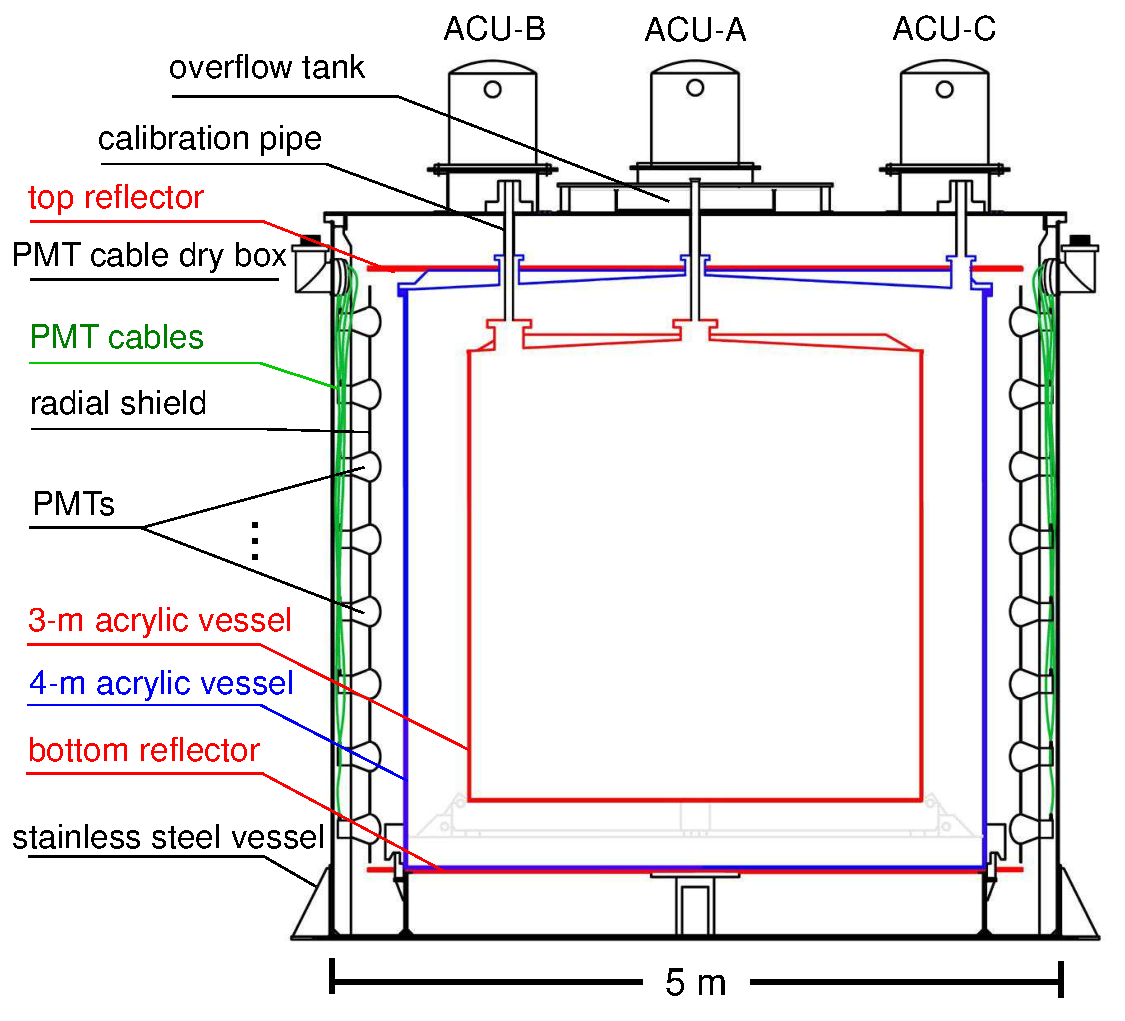
\includegraphics[scale=0.4]{exp_AD_structure.pdf}
  \caption{Structure of a Daya Bay antineutrino detector. From \cite{An_2017}.}
  \label{fig:expDetector}
\end{figure}


\subsection{Detection principle}
\label{sec:expDetPrinc}

\begin{figure}[ht]
  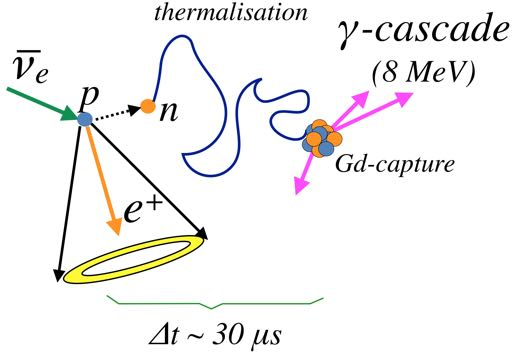
\includegraphics[scale=0.4]{ibd.png}
  \caption{The inverse beta decay reaction. Unlike a water Cerenkov detector, a Daya Bay AD cannot discern the direction of the positron. From \cite{Fernandez_2017}.}
  \label{fig:expIBD}
\end{figure}

\section{Shielding/vetoing system}
\label{sec:expShieldVeto}

\begin{figure}[ht]
  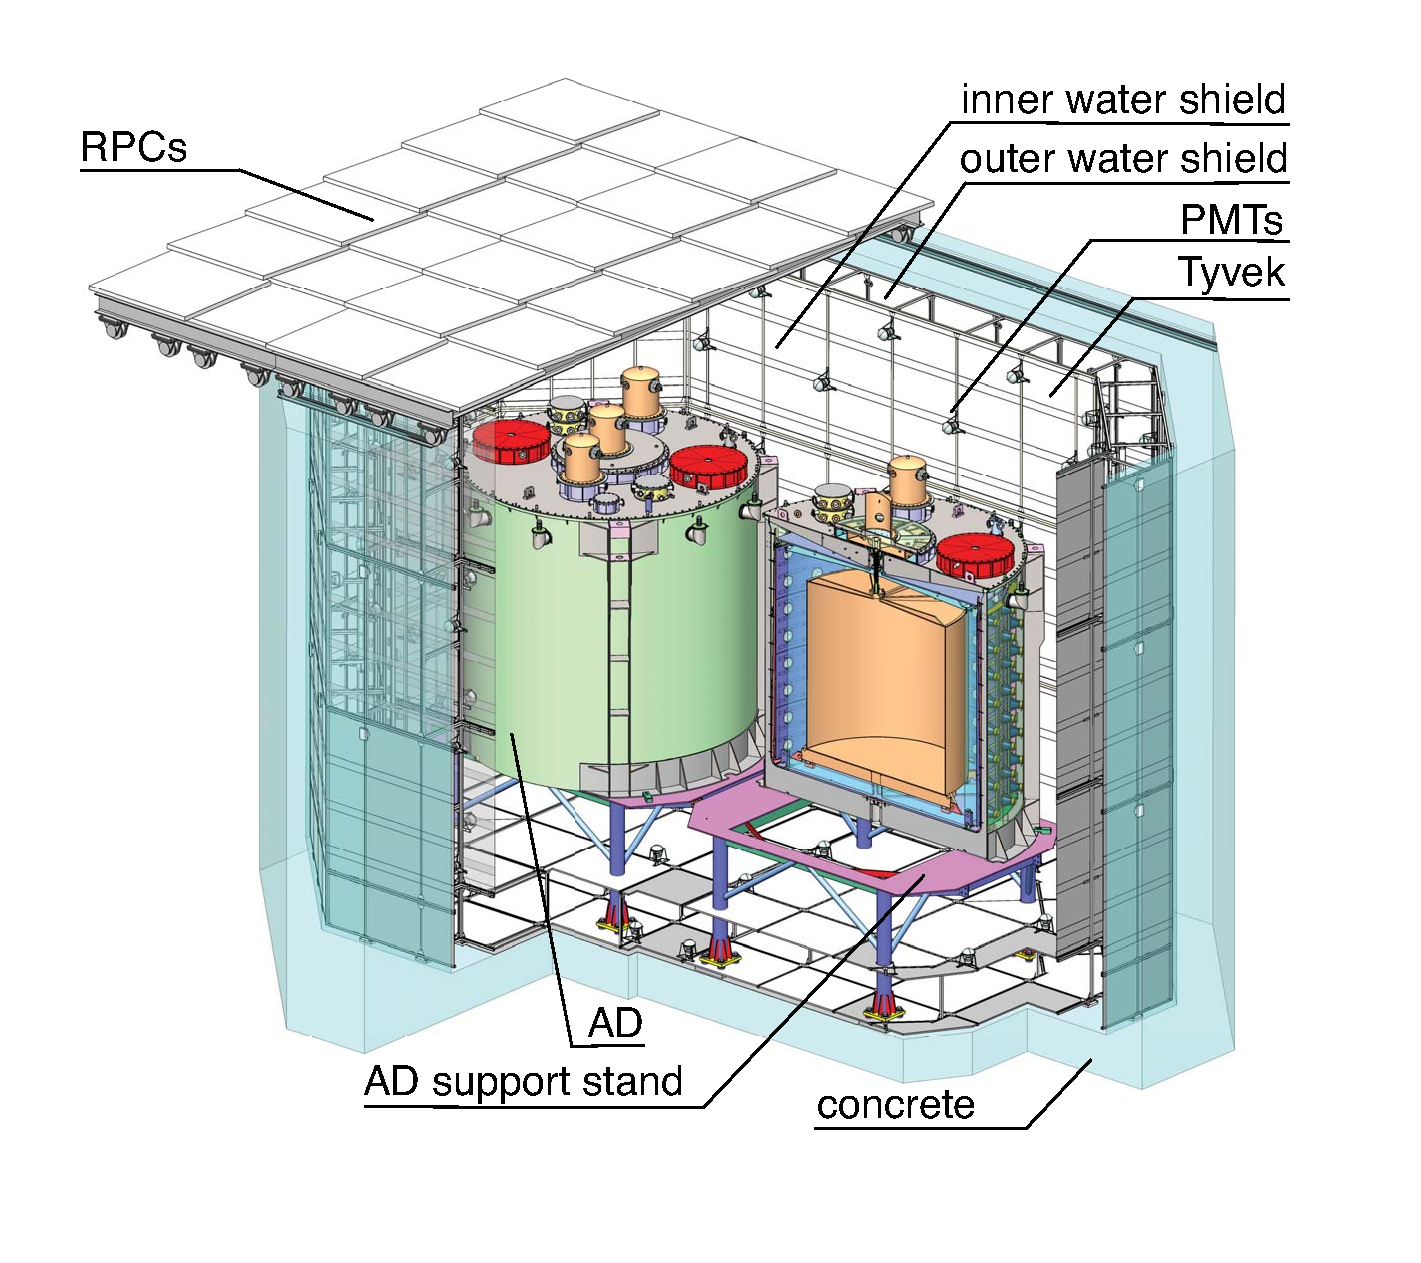
\includegraphics[scale=0.4]{exp_near_site_diagram.pdf}
  \caption{Water pool (including ADs) as configured in the near halls. The far hall is similar, with four ADs instead of two. From \cite{An_2017}.}
  \label{fig:expPool}
\end{figure}

\subfilebackmatter

\end{document}